\documentclass[pdf]{beamer}
\mode<presentation>{}
\usepackage{minted}
\usepackage{tikz}
\usepackage{pgffor} %% gives looping with \foreach
\usepackage[absolute,overlay]{textpos}
\usepackage{lmodern} %% scalable latin characters
\usetikzlibrary{arrows,shapes,backgrounds}
\usepackage{multirow}
\usepackage{listings} %% another package for code related stuff
\usepackage{hyperref}

%% stuff for minted
\definecolor{mintedBg}{rgb}{0.95, 0.95, 0.95}
\definecolor{blockBg}{rgb}{0.6, 0.6, 0.95}
\definecolor{rnaColor}{rgb}{0, 0.6, 0}
\definecolor{cdsColor}{rgb}{0, 0.4, 0.4}
\definecolor{rnaPol}{rgb}{0.8,0,0.8}
\definecolor{ribosomeCol}{rgb}{0.5,0.5,0.1}
\definecolor{protColor}{rgb}{0.6,0,0.6}
%% colours for nucleotides:
\definecolor{dACol}{rgb}{0.5, 0.5, 0}
\definecolor{dCCol}{rgb}{0.8, 0, 0}
\definecolor{dGCol}{rgb}{0, 0.8, 0}
\definecolor{dTCol}{rgb}{0, 0, 0.8}
    
%% define styles for different codes
\newminted{cpp}{linenos, bgcolor=blockBg, fontsize=\footnotesize}
%% then use \begin{cppcode}
\newminted{c}{linenos, bgcolor=mintedBg, fontsize=\footnotesize}
\newminted{perl}{linenos, bgcolor=mintedBg, fontsize=\footnotesize}

%% a command to define a subheading
\newcommand\subHeading[1]{
  \par\bigskip {\Large\bfseries#1}\par\smallskip
}

%% I detest indentation in footnotes etc, so try this:
\makeatletter
\renewcommand\@makefntext[1]{\noindent\makebox[0em][r]{\@makefnmark}\tiny#1}
\makeatother
%% the makeatletter and makeatother are required to allow me to
%% to change the macro beginning with an @. (though when I call it
%% I don't use the @ ... 

\setlength\parskip{0.5em}
\setlength\parindent{0ex}

%% to have footnotes without references. This from tex.stackexchange.com
\newcommand\blfootnote[1]{%
  \begingroup  %% this makes it a local redefinition
  \renewcommand\thefootnote{}\footnote{#1}%
  \addtocounter{footnote}{-1}  % this adjusts the footnote counter
  \endgroup
}


\title{Biological databases \& sequence formats}
\subtitle{How to get and look at data}
\author{Martin Jakt}

\begin{document}

\begin{frame}
  \titlepage
\end{frame}

\begin{frame}{Backends \& Frontends}
  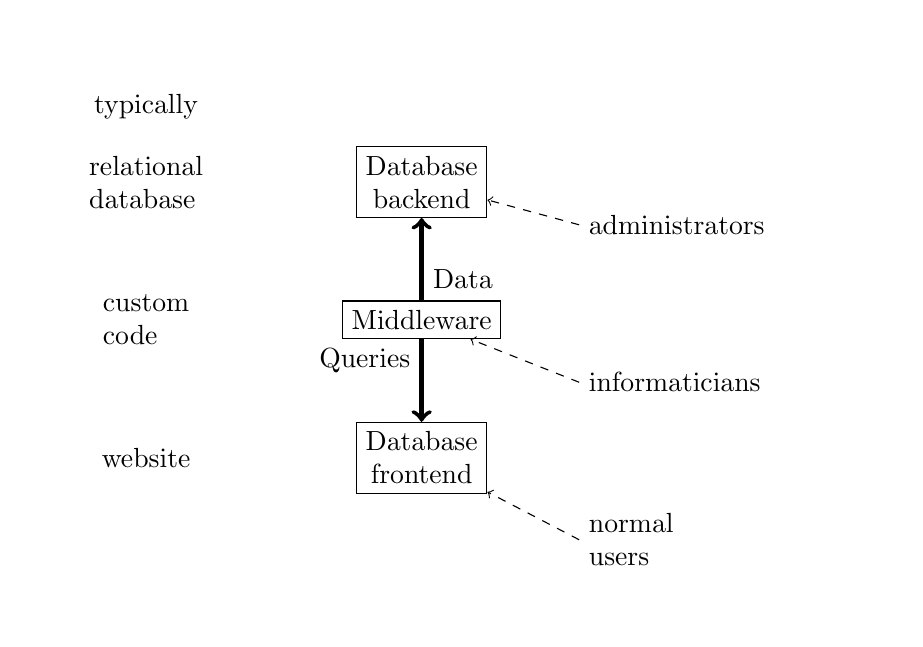
\begin{tikzpicture}[scale=0.5]
    \draw [help lines, opacity=0] (0,0) grid (22,15);
    %\foreach \x in {1,2,...,19} \node [font=\small] at (\x,0) {\x};
    %\foreach \y in {1,2,...,15} \node [font=\small] at (20,\y) {\y};
    \node [below, draw, align=center] (dbkend) at (10,12) {Database\\backend};
    \node [below, draw, align=center] (dfront) at (10,5) {Database\\frontend};

%    \draw [<->, ultra thick] (dbkend.south) -- (dfront.north) 
%    node [midway, left] {Queries}
%    node [midway, right] {Data};
    %% alternatively
    \draw [<->, ultra thick] (dbkend.south) -- (dfront.north) 
    node [pos=0.7, left] {Queries}
    node [pos=0.3, right] {Data};
    \pause
    \draw [] (dbkend.south) -- (dfront.north) 
    node [midway, fill=white, draw] (mware) {Middleware};
    \pause
    \draw (3,0 |- dbkend) node [align=left] (reldb) {relational\\database};
    \draw (3,0 |- mware) node [align=left] (ccode) {custom\\code};
    \draw (3,0 |- dfront) node [align=left] (wsite) {website};
    \draw (reldb |- 0,13) node [align=left] (timp) {typically};
%    \node [below, align=left, font=\small] at (3,0 |- dbkend.bottom) 
%    {typically\\relational\\database};
    \pause
    \draw [->, dashed] (14,2) node [right,align=left] {normal\\users} -- (dfront);
    \draw [->, dashed] (14,6) node [right,align=left] {informaticians} -- (mware);
    \draw [->, dashed] (14,10) node [right,align=left] {administrators} -- (dbkend);
  \end{tikzpicture}
\end{frame}

\begin{frame}{Types of databases}
  Types of databases (from a user perspective):\\
  {\small
  \begin{itemize}
    \item Sequences (non-curated)
    \item Sequences (curated to add annotation and reduce redundancy)
    \item Structures (mostly protein, primarily experimental data)
    \item Experimental data (difficult to structure)
      {\small
      \begin{itemize}
        \item Extract based expression analysis (quantitative)
        \item In situ based expression data (image based, qualitative)
        \item Phenotypes
        \item ...
      \end{itemize}
      }
    \item Data assemblies (multiple data types organised around a core concept)
    \item Specialised databases (eg. non-coding RNAs, immunoglobulin rearrangements)
    \item Reagents (eg. antibodies)
    \item literature (eg Pubmed)
    \item user generated (Wikis!)
  \end{itemize}
  \par
}
\end{frame}

\begin{frame}{Entrez}
  Access point to 39 different databases:\\
  
  {
    \bf \url{http://www.ncbi.nlm.nih.gov/}
  }
%  \href{http://www.ncbi.nlm.nih.gov/}{NCBI Entrez}
  
  Including:
  \begin{itemize}
    \item Genbank (nucleotide)
    \item Pubmed (abstracts)
    \item Gene expression (Gene Expression Omnibus: GEO)
    \item Probe (useful for experiments)
    \item Single nucleotide polymorphisms (SNP)
  \end{itemize}
  Some very useful stuff indeed.
\end{frame}

\begin{frame}{Entrez (2)}
  \small
  \begin{description}
    \item[NR4A2] A gene I have some historical interest in
  \vspace{-2ex}
  \end{description}
  \pause
%  \begin{figure}[ht] % this doesn't seem to do anything reasonable
    \begin{tikzpicture}[scale=0.5]
      \node [inner sep=0pt, above right] at (0,0)
      {\includegraphics[height=7.5cm]{images/Entrez_NR4A2.png}};
%      {\includegraphics[height=0.8\textheight]{images/Entrez_NR4A2.png}};
      \draw [help lines, opacity=0] (0,0) grid (22,15);
      %\foreach \x in {1,2,...,19} \node [font=\small] at (\x,0) {\x};
      %\foreach \y in {1,2,...,15} \node [font=\small] at (20,\y) {\y};
      \pause
      \node [inner sep=0pt, below right] at (0,15)
      {\includegraphics[width=3.79cm]{images/NR4A2_search_box}};
      \pause
      \node [inner sep=0pt, below right] (literature) at (0.25,13)
      {\includegraphics[width=5.33cm]{images/NR4A2_literature}};
      \node [right] at (literature.east) {Literature};
      \pause
      \node [inner sep=0pt, below right] (genomes) at (0.5,12)
      {\includegraphics[width=5.55cm]{images/NR4A2_genomes}};
      \pause
      \node [inner sep=0pt, below right] (genes) at (1,11)
      {\includegraphics[width=5.58cm]{images/NR4A2_genes}};
    \end{tikzpicture}
%  \end{figure}
\end{frame}

\begin{frame}{Entrez Literature}
  \begin{tikzpicture}[scale=0.5]
    \node [inner sep=0pt, above right] at (0,0)
    {\includegraphics[height=7.5cm]{images/NR4A2_pubmed}};
    \draw [help lines, opacity=0] (0,0) grid (22,15);
    %\foreach \x in {1,2,...,19} \node [font=\small] at (\x,0) {\x};
    %\foreach \y in {1,2,...,15} \node [font=\small] at (20,\y) {\y};
    \pause
    \node [inner sep=0pt, below right] at (0.5,14.5)
    {\includegraphics[width=6.79cm]{images/Nurr1_paper.png}};
    \pause
    \node [inner sep=0pt, above right] at (0,0)
    {\includegraphics[height=7.5cm]{images/Foxm1_Nr4a2_abstract}};
    
  \end{tikzpicture}
\end{frame}

\begin{frame}{Entrez Genomes}
      \begin{tikzpicture}[scale=0.5]
%      \node [inner sep=0pt, above right] at (0,0)
%      {\includegraphics[height=7.5cm]{images/Entrez_NR4A2.png}};
%      {\includegraphics[height=0.8\textheight]{images/Entrez_NR4A2.png}};
      \draw [help lines, opacity=0] (0,0) grid (22,15);
      %\foreach \x in {1,2,...,19} \node [font=\small] at (\x,0) {\x};
      %\foreach \y in {1,2,...,15} \node [font=\small] at (20,\y) {\y};
      \pause
      \node [inner sep=0pt, below right] (genomes) at (0,15)
      {\includegraphics[width=5.55cm]{images/NR4A2_genomes}};
      \pause
      \node [inner sep=0pt, below right] (nucleotides) at (0,15)
      {\includegraphics[height=7.5cm]{images/Nr4a2_nucleotide}};
      \pause
      \node [inner sep=0pt, below right] (human) at (0.5, 14.5)
      {\includegraphics[height=1.5cm]{images/Nr4a2_human}};
      \node [inner sep=0pt, below right] (predicted) at (0.5, 10.5)
      {\includegraphics[height=1.46cm]{images/Nr4a2_predicted}};
      \node [inner sep=0pt, below right] (synthetic) at (0.5, 6.5)
      {\includegraphics[height=1.39cm]{images/Nr4a2_synthetic}};
      
    \end{tikzpicture}
\end{frame}


\begin{frame}{Too many sequences?}
\begin{columns}[t]
  \begin{column}{0.5\textwidth}
    Bad?\\
    \vspace{2ex}
    Refine search.
    \vspace{1ex}
  \end{column}
  \begin{column}{0.5\textwidth}
    Good?\\
    \vspace{2ex}
    Lots of data that can be analysed.
  \end{column}
\end{columns}
\end{frame}


\begin{frame}{Refining the search}
  Options:\\
  { \tiny \href{http://www.ncbi.nlm.nih.gov/books/NBK3837/\#EntrezHelp.Entrez_Searching_Options}{www.ncbi.nlm.nih.gov/books/NBK3837/\#EntrezHelp.Entrez\_Searching\_Options} }
  \par
  Fields:\\
  { \tiny \href{http://www.ncbi.nlm.nih.gov/entrez/query/static/help/Summary_Matrices.html\#Search_Fields_and_Qualifiers}{www.ncbi.nlm.nih.gov/entrez/query/static/help/Summary\_Matrices.html\#Search\_Fields\_and\_Qualifiers} }

  \vspace{0.5cm}
  Boolean operators:\\
  {\setlength{\leftskip}{1cm}\small
    AND\\
    OR\\
    NOT\\
  }
  \vspace{0.5cm}
  eg:\\
  nr4a2 [GENE] AND mus musculus [ORGN] OR (nurr1 [GENE] AND mus musculus [ORGN])\\


  \blfootnote{I used Google to find the specific information after wasting time trying to find it by following links at the website}
\end{frame}

\begin{frame}{Sequence data annotation}
  Not just bags of sequences.
  \pause
  Metadata\footnote{information about the data}
  \pause
  \vspace{-2ex}
  \small
  \begin{description}
  \item[Identifier (1)] A common term (eg. gene or protein name, genomic location)
  \item[Who] Who created the data
  \item[When] When was the data created and added to the database
  \item[Type] What kind of data (DNA, RNA, Protein)
  \item[How] Sequence from (DNA, RNA, Protein)
  \item[Origin (2)] What kind of sample
    \begin{itemize}
    \item Species
    \item Tissue type
    \item Developmental stage
    \item Other conditions (eg. drug treatment / starvation)
    \end{itemize}
  \item[Identifier (2)] Unique identifer enabling cross-references
  \end{description}
  
\end{frame}

\begin{frame}{Sequence links}
  {\small
  \begin{description}
    \item[Human] \href{http://www.ncbi.nlm.nih.gov/nuccore/NM_006186.3}{www.ncbi.nlm.nih.gov/nuccore/NM\_006186.3}
    \item[Synthetic] \href{http://www.ncbi.nlm.nih.gov/nuccore/KJ897268.1}{www.ncbi.nlm.nih.gov/nuccore/KJ897268.1}
    \item[Predicted] \href{http://www.ncbi.nlm.nih.gov/nuccore/XM_005315789.1}{http://www.ncbi.nlm.nih.gov/nuccore/XM\_005315789.1}
  \end{description}
  }
  
  How to read and write Genbank / EMBL / DDBJ files:\\
  \url{http://www.insdc.org/documents/feature_table.html}
\end{frame}


\begin{frame}{Looking and editing genbank files}
  APE:\\
  A Plasmid Editor\\
  \url{http://biologylabs.utah.edu/jorgensen/wayned/ape/}

  Very useful and free application for manipulating sequnces.
  Especially when creating complex constructs.
\end{frame}

\begin{frame}{Nucleotide sequence databases}
  \begin{description}
    \item[Genbank] National Center for BioInformatics\\
      \url{http://www.ncbi.nlm.nih.gov/nuccore}
    \item[EMBL] European Molecular Biology Laboratory\\
      \url{http://www.ebi.ac.uk/ena}
    \item[DDBJ] DNA Data Bank of Japan\\
      \url{http://www.ddbj.nig.ac.jp}
  \end{description}
  
  These contain the same sequences, but have different interfaces and
  search implementations.\\
  Same search $\Rightarrow$ different results.

  Mostly a personal preferences which to use. Explore at your leisure.

  EMBL files has a different sequence format eg.\\
  {\footnotesize
  \url{http://www.ebi.ac.uk/ena/data/view/AB590645&display=text}
  }
\end{frame}

\begin{frame}[fragile]{fasta: the universal sequence format}
  Very lightweight format. Easy to read and write by hand or script.\\
  Can contain multiple sequences.
  \begin{verbatim}
    >seq1_identifier optional description
    ACTAGATACTATACATACATACCCGAGATACATGACTAGACTAA
    ACGGACTACGATACATACGATATA
    >seq2_identifier optional description
    GACTAGACTACTACGATAAGATAACCAATATACAGAACTACTAC
    ACGATAACGATACGTACGGATTACTAGACTACCGATACGGATACTAG
  \end{verbatim}
  {\small
  \begin{itemize}
    \item Header line begins with \verb|'>'| immediately followed by a unique identifer.
      Text following the identifier on same line can provide additional description.
    \item The sequence is written in the lines following a header line. These should
      contain only sequence data. The sequence ends at the next header line.
  \end{itemize}
  }
\end{frame}

\begin{frame}[fragile]{fastq: the NGS format}
  Contains both sequence and quality scores.\\
  Usually thousands to millions of sequences in a single file.
  {\footnotesize
  \begin{verbatim}
@SEQ_ID
GATTTGGGGTTCAAAGCAGTATCGATCAAATAGTAAATCCATTTGTTCAACTCACAGTTT
+
!''*((((***+))%%%++)(%%%%).1***-+*''))**55CCF>>>>>>CCCCCCC65
  \end{verbatim}
    }
  Lines are:
  \begin{enumerate}
    \item Sequence identifier after \verb|@| (must be unique)
    \item Sequence (usually no newlines)
    \item \verb|+| optionally followed by the identifier
    \item A quality string of the same length as the sequence, indicating the
      probabilities of each base being miscalled.
  \end{enumerate}
  \blfootnote{\url{https://en.wikipedia.org/wiki/FASTQ_format}}
\end{frame}

\begin{frame}[fragile]{fastq quality scores}
  Quality is usually defined as:
  $$
  Q = -10\log_{10}e
  $$
  where $e$ is the estimated probability that the base call is wrong.
  \pause
  The quality values are encoded using a subset of the ASCII code:
  {\tiny
\begin{verbatim}
  SSSSSSSSSSSSSSSSSSSSSSSSSSSSSSSSSSSSSSSSS.....................................................
  ..........................XXXXXXXXXXXXXXXXXXXXXXXXXXXXXXXXXXXXXXXXXXXXXX......................
  ...............................IIIIIIIIIIIIIIIIIIIIIIIIIIIIIIIIIIIIIIIII......................
  .................................JJJJJJJJJJJJJJJJJJJJJJJJJJJJJJJJJJJJJJJ......................
  LLLLLLLLLLLLLLLLLLLLLLLLLLLLLLLLLLLLLLLLLL....................................................
  !"#$%&'()*+,-./0123456789:;<=>?@ABCDEFGHIJKLMNOPQRSTUVWXYZ[\]^_`abcdefghijklmnopqrstuvwxyz{|}~
  |                         |    |        |                              |                     |
 33                        59   64       73                            104                   126
  0........................26...31.......40                                
                           -5....0........9.............................40 
                                 0........9.............................40 
                                    3.....9.............................40 
  0.2......................26...31........41                              

 S - Sanger        Phred+33,  raw reads typically (0, 40)
 X - Solexa        Solexa+64, raw reads typically (-5, 40)
 I - Illumina 1.3+ Phred+64,  raw reads typically (0, 40)
 J - Illumina 1.5+ Phred+64,  raw reads typically (3, 40)
     with 0=unused, 1=unused, 2=Read Segment Quality Control Indicator (bold) 
     (Note: See discussion above).
 L - Illumina 1.8+ Phred+33,  raw reads typically (0, 41)
\end{verbatim} }
    \blfootnote{\url{https://en.wikipedia.org/wiki/FASTQ_format}}
\end{frame}

\begin{frame}{Genome databases}
  Mapping sequences to genomes allows redundancy to be collapsed and information
  to be summarised.

  \begin{itemize}
    \item UCSC (University of California Santa Cruz) Genome Bioinformatics
      \url{https://genome.ucsc.edu/}
    \item Ensembl (joint project between EMBL-EBI and the Wellcome Trust Sanger Institute)
      \url{http://www.ensembl.org/index.html}
  \end{itemize}
  
  Information about gene structure, genome features and sequence variation organised
  by genome location.

  Orthology across species predefined allowing interesting analyses.

  Again, mostly personal choice as to which you use.
\end{frame}

\begin{frame}{Gene Function}
  \begin{description}
    \item[Human:] OMIM, Online Mendelian Inheritance in Man\\
      \url{http://omim.org/entry/601828}\\
    \item[Mouse:] MGI, Mouse Genome Informatics\\
      \url{http://www.informatics.jax.org/}
    \item[Zebra fish] ZFIN\\
      \url{http://zfin.org/}
  \end{description}
  
  Rich sources of information.
\end{frame}

\begin{frame}{Protein data}
  UniProt

  \url{http://www.uniprot.org/}

  Both automatically annotated and manually curated data available.\\
  \vspace{1ex}
  eg. VEGFR2 :\\
  {\small
  \url{http://www.uniprot.org/uniprot/?query=vegfr2&sort=score}
}
\end{frame}

\begin{frame}{Protein domains and families}
  \begin{description}
    \item[Prosite]
      \url{http://prosite.expasy.org/}  
    \item[Pfam]
      \url{http://pfam.xfam.org/}
    \item[Interpro]
      \url{http://www.ebi.ac.uk/interpro/}
  \end{description}

  Cover different but related aspects of protein domain structure.
\end{frame}

\begin{frame}{Gene expression data}
  \begin{description}
    \item[Gene Expression Omnibus] GEO, the NCBI implementation\\
      \url{http://www.ncbi.nlm.nih.gov/geo/}
    \item[ArrayExpress] The EBI implementation\\
      \url{https://www.ebi.ac.uk/arrayexpress/}
  \end{description}
  
  For these the difficulty lies in the description of experimental
  details and in comparing data across several data sets.
\end{frame}

\begin{frame}{Taxonomy}
  Another NCBI database:

  \url{http://www.ncbi.nlm.nih.gov/guide/taxonomy/}

\end{frame}

\begin{frame}{Taxonomy (2)}
  I don't like web interfaces:
  \begin{enumerate}
  \item Downloaded database (flat files, but relational)
  \item Wrote script to browse and extract species
  \item $\rightarrow$ automate sequence retrieval
  \item $\rightarrow$ automate phylogenetic analysis
  \end{enumerate}
  
  NCBI provide a web-API that makes it reasonably easy to write scripts to
  download specific sequences. This allows you to combine the information in
  the different databases without inducing RSI.

\end{frame}

\begin{frame}{and lots more...}
  The 2015 \emph{Nucleic Acids Research} Database Issue
  and Molecular Biology Database Collection\\
  {\small
    \url{http://nar.oxfordjournals.org/content/43/D1/D1.full}
  }

  \begin{itemize}
  \item 56 new databases
  \item 115 updates
  \end{itemize}
  
\end{frame}
\end{document}
